% ACCV 2026 format.
% Requires: llncs.cls (texlive-publishers or https://www.springer.com/gp/computer-science/lncs/conference-proceedings-guidelines)
%           accv2026.sty (from https://accv2026.org/submission when released)
\documentclass[runningheads]{llncs}

\usepackage[numbers]{natbib}
% Math commands
\newcommand{\R}{\mathbb{R}}
\newcommand{\E}{\mathbb{E}}
\newcommand{\Pb}{\mathbb{P}}
\newcommand{\calX}{\mathcal{X}}
\newcommand{\calY}{\mathcal{Y}}
\newcommand{\calD}{\mathcal{D}}
\newcommand{\calB}{\mathcal{B}}
\newcommand{\idonly}{\texttt{id\_only}}
\newcommand{\mixed}{\texttt{mixed}}
\newcommand{\nota}{\texttt{no\_tta}}
\newcommand{\ml}{\texttt{mixed\_maskedloss}}
\newcommand{\idfull}{\texttt{id\_fullmatch}}
\newcommand{\idsub}{\texttt{id\_subbatch}}
\newcommand{\DeltaA}{\Delta\text{AUROC}}
\newcommand{\gap}{\Delta_{\text{gap}}}
\newcommand{\forfeit}{f_\alpha}
% Shorthand
\newcommand{\eg}{\textit{e.g.},}
\newcommand{\ie}{\textit{i.e.},}
\newcommand{\cf}{\textit{cf.}~}
\newcommand{\etal}{\textit{et al.}}


\usepackage{hyperref}
\usepackage{url}
\usepackage{booktabs}
\usepackage{graphicx}
\usepackage{amsmath,amssymb}
\usepackage{xcolor}
\usepackage{microtype}
\usepackage{subcaption}
\usepackage{multirow}
\usepackage{array}
\usepackage{enumitem}
% LLNCS-native theorem definition (no amsthm needed)
\spnewtheorem{observation}{Observation}{\bfseries}{\itshape}

\title{Open-World TTA Safety: Entropy Minimization Forfeits OOD Detection Gain and Inverts Method Rankings}
\titlerunning{Open-World TTA Safety}

\author{Anonymous}
\authorrunning{Anonymous}
\institute{Anonymous Institution}

\begin{document}

\maketitle

\begin{abstract}
We show that standard closed-set TTA rankings actively invert open-world safety rankings.
In our heavy-contamination audit ($\alpha{=}0.9$, averaged across OOD datasets and corruptions), ETA ranks first by ID-accuracy gain but joint-last by mixed-stream AUROC, and the no-adaptation baseline attains higher open-world OOD detection than any entropy-minimizing TTA method tested.
This reversal arises because entropy-minimizing TTA sharpens predictions on \emph{all} inputs---including OOD inputs whose uncertainty should be preserved---creating an objective-level conflict with OOD detection.
We introduce a \emph{paired contamination protocol} that isolates this conflict experimentally, pairing an ID-only oracle against realistic mixed-batch adaptation on identical test streams.
Across 4 OOD datasets, 2 TTA methods, 4 ID fractions, and 3 OOD detectors, the oracle consistently outperforms the realistic baseline (27/32 cells, $p < 0.05$), with contamination forfeiting up to 289\% of the achievable OOD-detection benefit.
A four-condition mechanistic decomposition identifies \emph{OOD gradient contamination} as the dominant driver: including OOD samples in the entropy loss collapses the ID/OOD score gap, while BatchNorm exposure to OOD inputs (without the gradient) is actively beneficial.
We replicate these findings at ImageNet scale (8/8 cells, ResNet-50, NINCO) and recommend paired-gap reporting as a required evaluation column for TTA papers targeting open-world deployment.
\keywords{test-time adaptation \and out-of-distribution detection \and open-world evaluation \and entropy minimization \and paired protocol}
\end{abstract}

\section{Introduction}
\label{sec:intro}

Test-time adaptation (TTA) corrects for distribution shift by updating a model's parameters online using only unlabeled test data.
The dominant evaluation protocol measures how much closed-set accuracy improves on corrupted in-distribution images.
This metric answers one question well: \emph{does the model classify shifted images more accurately after adaptation?}
It is blind to a second question that matters equally in real deployment: \emph{does the model still know what it does not know?}

In realistic deployment, test streams are not curated.
Batches mix corrupted in-distribution (ID) samples with out-of-distribution (OOD) samples from categories the model has never seen.
A model must simultaneously (1) classify shifted ID images correctly---what TTA optimizes---and (2) detect OOD images as anomalous and abstain.
Entropy-minimizing TTA \citep{tent} pursues objective (1) by sharpening every prediction toward its current most likely class.
This conflicts directly with objective (2): sharpening OOD predictions eliminates the uncertainty that OOD detectors rely on.

\begin{figure}[t]
  \centering
  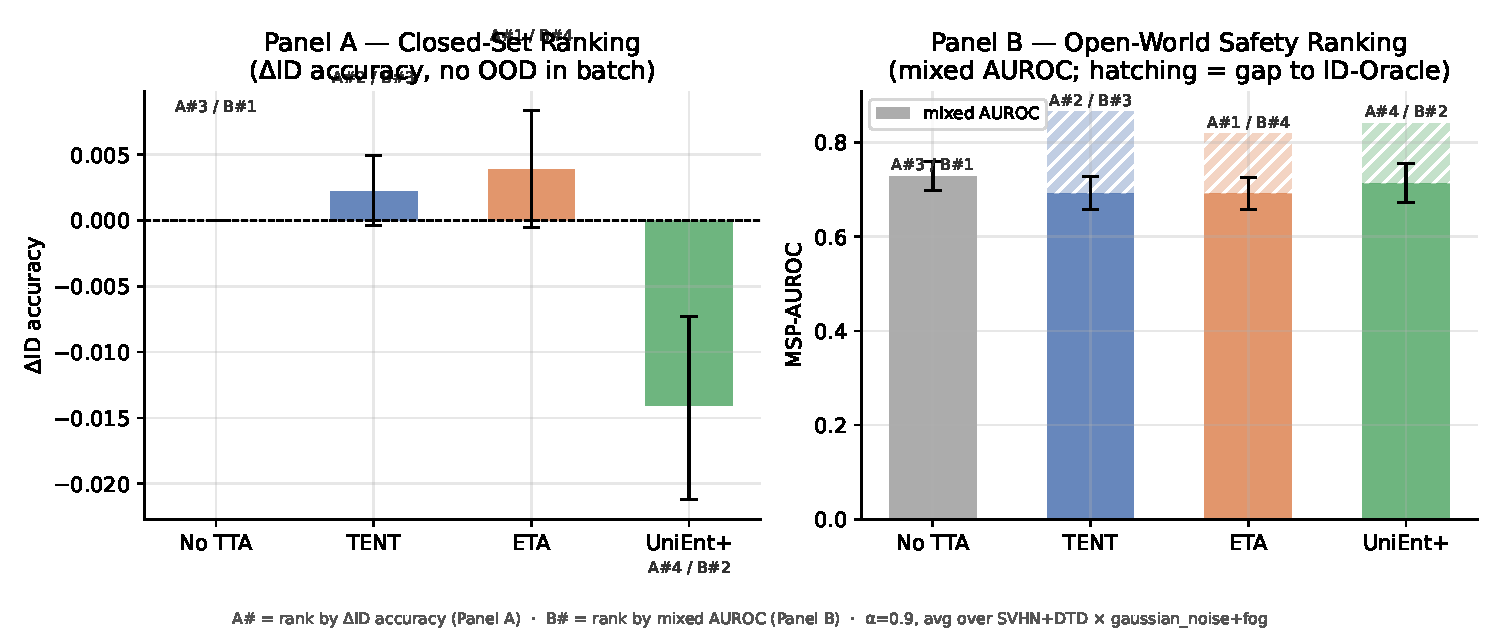
\includegraphics[width=\linewidth]{figures/fig1_ranking_reversal.pdf}
  \caption{%
    \textbf{Closed-set TTA rankings invert open-world safety rankings.}
    \emph{Left (Panel A)}: Closed-set metric---change in ID accuracy on corrupted CIFAR-10 ($\alpha{=}0.9$, gaussian noise). ETA ranks first, UniEnt+ last.
    \emph{Right (Panel B)}: Open-world metric---mixed-stream AUROC. No adaptation ranks first; ETA and TENT fall \emph{below} the no-adaptation baseline. The method that tops the closed-set leaderboard (ETA) ranks joint-last by open-world AUROC (averaged at $\alpha{=}0.9$).
    Rank numbers overlaid on each bar.
  }
  \label{fig:ranking_reversal}
\end{figure}

Prior work on open-world TTA \citep{owttt,unient,rosetta} acknowledges that OOD contamination degrades adaptation quality and proposes methods to mitigate it.
We ask a different question: \emph{how much does each method actually solve?}
We introduce a \emph{paired contamination protocol} that measures this directly, and apply it as a diagnostic across existing methods including those explicitly designed for open-world settings.

\paragraph{Contributions.}
\begin{enumerate}[leftmargin=*,topsep=2pt,itemsep=1pt]
  \item \textbf{Paired contamination protocol.} We define a contamination cost $\gap = \DeltaA(\idonly) - \DeltaA(\mixed)$ by pairing an ID-only oracle against realistic mixed-batch adaptation on identical test streams. The forfeit fraction $\forfeit = \gap / \DeltaA(\idonly)$ measures what fraction of the achievable OOD-detection benefit is lost to contamination. Across 4 OOD datasets, 2 TTA methods, 4 ID fractions $\alpha$, and 3 OOD detectors, the gap is significant in 27/32 cells ($p < 0.05$); $\forfeit > 1$ in most cells, meaning mixed TTA leaves OOD detection \emph{worse} than no adaptation.

  \item \textbf{Mechanism decomposition.} A four-condition experimental control isolates OOD gradient contamination as the dominant mechanism (+120--456\% of the total gap). BatchNorm statistics exposure to OOD inputs, decoupled from the gradient, is not harmful---it is actively beneficial. This overturns the prior hypothesis that shared batch statistics are the culprit.

  \item \textbf{Cross-method safety audit.} Applying the paired protocol across four method families---No TTA, TENT, ETA, and UniEnt+---reveals a ranking reversal: ETA ranks first by closed-set ID-accuracy gain but joint-last by mixed-stream AUROC (tied with TENT). In our heavy-contamination audit ($\alpha = 0.9$, averaged across OOD datasets and corruptions), the no-adaptation baseline attains the highest mixed-stream AUROC, exceeding all entropy-minimizing TTA methods tested. UniEnt+, designed explicitly for open-world streams, partially recovers but does not close the gap.

  \item \textbf{Reporting standard.} We recommend that TTA papers targeting open-world deployment report the paired contamination gap alongside ID accuracy, making the adaptation--abstention tradeoff visible.
\end{enumerate}

\paragraph{Scope and limitations.} The \idonly{} oracle is a diagnostic tool, not a deployable method: it requires ground-truth ID/OOD labels---precisely what an OOD detector is designed to produce. Our contribution is the gap $\gap$ as an interpretable bound, not a system one can deploy. We do not propose a new adaptation algorithm; we provide the evaluation tool that reveals how much each existing algorithm actually solves. Limitations are discussed in Section~\ref{sec:conclusion}.

\section{Background and Related Work}
\label{sec:background}

\paragraph{Entropy-minimizing TTA.}
Test-time adaptation updates model parameters using only the unlabeled test batch.
TENT \citep{tent} minimizes the mean per-sample softmax entropy over BatchNorm affine parameters.
ETA \citep{eta} adds an entropy threshold that filters high-entropy samples before computing the gradient, and a Fisher-regularized weight update.
SAR \citep{sar} and CoTTA \citep{cotta} extend these ideas to continual and non-stationary streams.
A common property of all entropy-minimizing methods is that they are \emph{class-closing}: the gradient sharpens each prediction toward its current argmax class, regardless of whether that class is semantically meaningful for the input.
This is well-suited to corrupted ID images, where the correct class is likely already the argmax, but it is adversarial to OOD detection, where the model's uncertainty should be preserved.

\paragraph{Score-based OOD detection.}
The maximum softmax probability (MSP) \citep{msp}, energy score \citep{energy}, and Mahalanobis distance \citep{mahal} all rely on the model expressing lower confidence or higher uncertainty on OOD inputs than on ID inputs.
MSP is low when the prediction is uncertain; energy is high when logits are spread; Mahalanobis distance is large when features are far from training-class prototypes.
All three are adversarially affected by entropy minimization: sharpening OOD predictions raises MSP, concentrates logits, and contracts features toward prototypes.

\paragraph{Open-world and open-set TTA.}
Several recent works address OOD contamination in TTA.
OWTTT \citep{owttt} extends TTA to open-world streams by detecting and clustering novel categories, framing contamination as a problem for a richer adaptation algorithm.
UniEnt and UniEnt+ \citep{unient} propose a unified entropy objective that applies entropy minimization to pseudo-ID samples and entropy maximization to pseudo-OOD samples, addressing the ID/OOD split at the loss level.
Concurrent with our work, ROSETTA \citep{rosetta} studies the same open-set TTA setting and proposes a mitigation method for the ID/OOD tradeoff.
These works confirm that the conflict exists and propose methods to reduce it.

Our work is complementary rather than algorithmic: we do not claim to discover this conflict or to solve it with a new adaptation rule.
Instead, we introduce a method-agnostic \emph{paired counterfactual protocol} and a four-condition mechanistic decomposition that quantify residual contamination cost for \emph{any} OSTTA method---including future ones.
This diagnostic asks a different question from absolute mixed-stream AUROC or ID accuracy: given a fixed test stream, how much OOD-detection improvement was achievable but forfeited because OOD samples entered the adaptation pathway?
We evaluate UniEnt+ under our protocol and show that the paired gap persists, partially reduced but not eliminated, demonstrating that the closed-set evaluation norm under-reports residual OOD-safety failures even for methods explicitly designed for open-world streams.
Evaluating ROSETTA under this protocol is an important next step; we do not include it here because the work appeared concurrently and no official implementation was available at our submission cutoff.
The distinction from ROSETTA and UniEnt is not ``we discovered the conflict'' but ``we provide the tool that measures what remains unsolved.''
ROSETTA strengthens the motivation for our protocol rather than subsuming it: once multiple OSTTA methods exist, the field needs a common diagnostic of residual contamination cost, not only absolute performance tables.

\paragraph{Evaluation in TTA.}
Standard TTA evaluation measures top-1 accuracy on corrupted ID images, typically from CIFAR-10-C \citep{imagenetc} or ImageNet-C \citep{imagenetc}.
Several papers note that TTA can fail silently---degrading performance on some samples while improving on others \citep{cotta,sar}---but these analyses remain within the closed-set ID-accuracy framework.
We extend this critique to a second axis: OOD safety.

\section{The Paired Contamination Protocol}
\label{sec:protocol}

\subsection{Problem Setup}

Let $f_\theta : \calX \to \R^C$ be a classifier with parameters $\theta$.
At test time, batches $\calB = \calB_{\text{ID}} \cup \calB_{\text{OOD}}$ arrive sequentially, where $|\calB_{\text{ID}}| = \alpha B$ and $|\calB_{\text{OOD}}| = (1-\alpha)B$ for batch size $B$ and ID fraction $\alpha \in (0,1)$.
$\calB_{\text{ID}}$ contains corrupted images from the source distribution; $\calB_{\text{OOD}}$ contains images from an entirely different category set.
The ID fraction $\alpha$ is unknown to the model.

TENT \citep{tent} updates the BatchNorm affine parameters $\gamma, \beta$ by minimizing:
\begin{equation}
  \mathcal{L}_{\text{TENT}} = \frac{1}{|\calB|} \sum_{x \in \calB} H(p_x), \quad H(p) = -\sum_c p_c \log p_c
  \label{eq:tent_loss}
\end{equation}
where $p_x = \text{softmax}(f_\theta(x))$.
Since $H(p)$ is minimized when $p$ is one-hot, this gradient sharpens every prediction toward its current argmax class.
OOD detectors such as MSP $= \max_c p_c$ rely on OOD inputs having \emph{low} $\max_c p_c$.
The objectives are in direct conflict on OOD samples in $\calB_{\text{OOD}}$.

\begin{observation}
\label{obs:conflict}
For uncertainty-based OOD detectors of the kind studied here, applying entropy minimization indiscriminately to mixed ID/OOD batches increases confidence on OOD samples as well as ID samples, tending to collapse the ID/OOD score gap unless OOD samples are excluded from the adaptation loss.
\end{observation}

\subsection{Paired Contamination Protocol}

We define three conditions applied to the same drawn batch $\calB$:

\begin{itemize}[leftmargin=*,topsep=2pt,itemsep=1pt]
  \item $\nota$: evaluate at $t=0$, no adaptation. Measures pre-adaptation AUROC.
  \item $\idonly$: adapt using $\mathcal{L}_{\text{TENT}}$ on $\calB_{\text{ID}}$ only. Requires ground-truth ID/OOD labels (oracle; unrealizable in deployment).
  \item $\mixed$: adapt using $\mathcal{L}_{\text{TENT}}$ on the full $\calB$. Realistic deployment condition.
\end{itemize}

The same random seed draws identical batches across all three conditions.
We run $n = 30$ independent batch draws per experimental cell and report:
\begin{align}
  \DeltaA(\cdot) &= \text{AUROC}(T) - \text{AUROC}(0) \label{eq:delta_auroc}\\
  \gap &= \DeltaA(\idonly) - \DeltaA(\mixed) \label{eq:gap}\\
  \forfeit &= \gap / \DeltaA(\idonly) \label{eq:forfeit}
\end{align}
with 95\% bootstrap CIs and a paired $t$-test.
The gap $\gap$ is the contamination cost: how much OOD-detection improvement is forfeited by using the full mixed batch instead of the clean ID oracle.
The forfeit fraction $\forfeit > 1$ indicates that mixed adaptation leaves OOD detection \emph{worse} than no adaptation.

\paragraph{The id-only oracle.}
$\idonly$ TENT is a diagnostic oracle, not a deployable method.
It requires ground-truth knowledge of which samples are ID versus OOD---precisely what an OOD detector is designed to produce.
Its role is to establish a measurable upper bound on OOD-detection improvement under zero contamination, providing a calibrated reference for the contamination cost.

\subsection{Four-Condition Mechanistic Decomposition}

To isolate the dominant mechanism, we introduce four conditions that incrementally add contamination components:

\begin{itemize}[leftmargin=*,topsep=2pt,itemsep=1pt]
  \item $\idsub$: adapt on ID slice of size $\alpha B$ (oracle, count-matched).
  \item $\idfull$: pad with extra corrupted ID images to full size $B$ (count control).
  \item $\ml$: forward pass on full $\calB$ (BatchNorm sees all images, including OOD), but entropy loss computed only on $\calB_{\text{ID}}$.
  \item $\mixed$: forward pass and entropy loss on full $\calB$ (realistic).
\end{itemize}

The additive decomposition is:
\begin{equation}
  \underbrace{\DeltaA(\idsub) - \DeltaA(\mixed)}_{\text{total gap}}
  = \underbrace{[\idsub - \idfull]}_{\text{sample-count artifact}}
  + \underbrace{[\idfull - \ml]}_{\text{BN statistics}}
  + \underbrace{[\ml - \mixed]}_{\text{OOD gradient}}
  \label{eq:decomp}
\end{equation}

This design separates three contamination sources: (1) the OOD batch being smaller than the full batch by $(1-\alpha)B$ samples, (2) BatchNorm computing joint statistics over ID and OOD images, and (3) OOD samples contributing to the entropy gradient.
The sample-count artifact is measured as $+3$--$12\%$ of the total gap, confirming that batch-size confounds are small and the protocol is fair.

\section{Contamination Cost: Characterization}
\label{sec:characterization}

\subsection{Setup}

\textbf{Model.} ResNet-18 \citep{resnet} trained on CIFAR-10 (95.14\% test accuracy).
BatchNorm affine parameters adapted by TENT; all other weights frozen.

\textbf{Corruption.} CIFAR-10-C \citep{imagenetc} at severity 5 (gaussian noise as main corruption; fog, impulse noise, elastic transform, and pixelate for generalization).

\textbf{OOD datasets.} SVHN \citep{svhn}, DTD \citep{dtd}, Places365 \citep{places365}, and CIFAR-100 \citep{cifar100}.
ID fraction $\alpha \in \{0.9, 0.75, 0.5, 0.25\}$.

\textbf{OOD detectors.} Maximum softmax probability (MSP) \citep{msp}, energy score \citep{energy}, Mahalanobis distance \citep{mahal}, KNN ($k{=}50$) \citep{knn_ood}, and ViM \citep{vim}. KNN and ViM results are in Sections~\ref{sec:characterization}--\ref{sec:recalibration}; the 27/32 significance count uses MSP, Energy, and Mahalanobis as primary detectors.

\textbf{TTA methods.} TENT \citep{tent} and ETA \citep{eta}; $T=10$ steps per batch. Extended method coverage (SAR, CoTTA, UniEnt+) is in Section~\ref{sec:audit}.

\textbf{Evaluation contract.} All OOD detectors are calibrated once on 10K source-domain training samples under the pretrained model and held fixed throughout adaptation (frozen-detector contract, see Section~\ref{sec:protocol}). For Mahalanobis distance, class means and precision matrix are computed from pretrained features and not updated. For KNN ($k{=}50$), training features are extracted from the pretrained model and frozen. This contract measures system-level compatibility between TTA and a pre-deployed detector not co-maintained during adaptation. We evaluate the recalibrated-detector contract in Section~\ref{sec:recalibration}.

\subsection{Core Result: Paired Contamination Gap}

\begin{figure}[t]
  \centering
  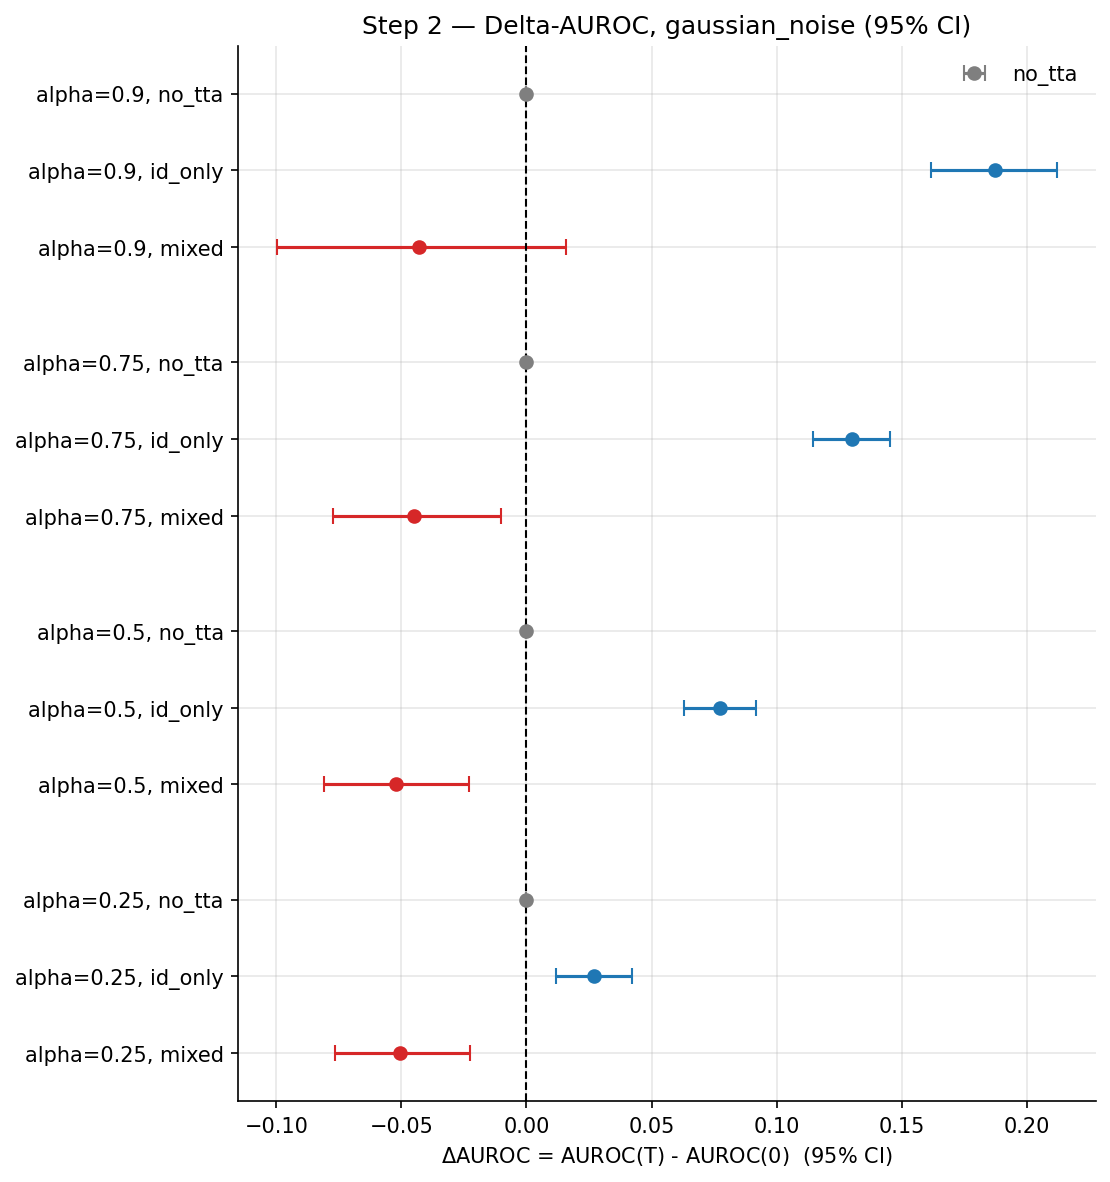
\includegraphics[width=0.7\linewidth]{figures/fig2_forest.png}
  \caption{%
    \textbf{Paired contamination gap across ID fractions $\alpha$ (SVHN OOD, gaussian noise, MSP-AUROC).}
    Mean $\DeltaA$ with 95\% bootstrap CIs for \nota{} (gray), \idonly{} (blue), and \mixed{} (red).
    The gap between \idonly{} and \mixed{} is significant at all $\alpha$ values ($p < 10^{-5}$).
    At $\alpha \le 0.75$, mixed TENT is worse than no adaptation (red below gray dashed).
  }
  \label{fig:forest}
\end{figure}

Figure~\ref{fig:forest} shows the core result for SVHN.
At $\alpha = 0.9$ (90\% ID), \idonly{} achieves $\DeltaA = +0.188$ while \mixed{} achieves $-0.043$: a gap of $+0.231$ ($p = 2.6 \times 10^{-8}$, forfeit fraction $= 1.23$).
At $\alpha = 0.5$, \idonly{} achieves $+0.077$ while \mixed{} achieves $-0.052$: an absolute gap of $+0.129$, corresponding to a forfeit fraction of $1.68$ (mixed TTA makes OOD detection \emph{worse} by 168\% of what ID-only TTA would have gained).

Table~\ref{tab:significance_summary} summarizes significance across all 32 experimental cells.
Individual cell $p$-values are Benjamini-Hochberg FDR-corrected across all 32 tests at $q = 0.05$; the 27/32 count holds under correction.

\begin{table}[t]
\centering
\small
\caption{%
  Significance of paired contamination gap ($\idonly{} > \mixed{}$, $p < 0.05$) across OOD datasets and TTA methods.
  Count = significant cells out of 4 ($\alpha \in \{0.9, 0.75, 0.5, 0.25\}$, gaussian noise, MSP-AUROC, $n=20$).
  27 of 32 cells are significant; non-significant cells are exclusively at $\alpha = 0.25$.
}
\label{tab:significance_summary}
\begin{tabular}{lcc}
\toprule
OOD Dataset & TENT & ETA \\
\midrule
SVHN         & 4/4 & 4/4 \\
DTD          & 4/4 & 4/4 \\
Places365    & 3/4 & 3/4 \\
CIFAR-100    & 2/4 & 3/4 \\
\midrule
\textbf{Total} & \textbf{13/16} & \textbf{14/16} \\
\bottomrule
\end{tabular}
\end{table}

\paragraph{Detector breadth (confidence-based and feature-based detectors).}
The paired gap holds across all three OOD detectors tested---MSP, energy, and Mahalanobis---all of which rely on logit-scale confidence or feature-space proximity (see Section~\ref{sec:background}).
For DTD at $\alpha = 0.9$: MSP gap $+0.212$ ($p = 7.9 \times 10^{-11}$), Energy gap $+0.225$ ($p = 1.7 \times 10^{-12}$), Mahalanobis gap $+0.031$ ($p = 2.9 \times 10^{-4}$).
Even for Mahalanobis, where corruption alone collapses AUROC by 0.58 before any adaptation, the contamination adds an incremental penalty above the corruption baseline.

\paragraph{Non-logit-scale detectors: KNN and ViM.}
We extend the detector evaluation to two non-logit-scale detectors that cannot be directly sharpened by entropy minimization: $k$-NN distance in L2-normalized feature space \citep{knn_ood} (KNN, $k{=}50$) and the ViM residual-norm score in the feature null space \citep{vim}.
Training features (10K samples from the source domain) are extracted once from the frozen pretrained model and held fixed.

Results at $\alpha = 0.9$, averaged over SVHN and DTD (gaussian noise and fog):

\begin{itemize}[leftmargin=*,topsep=2pt,itemsep=1pt]
  \item \textbf{KNN}: id-only AUROC exceeds mixed AUROC by $+0.061$ for TENT ($p = 6.7 \times 10^{-8}$) and $+0.036$ for ETA ($p = 1.2 \times 10^{-6}$). FPR95 follows the same direction (id-only FPR95 lower by $5.0\%$/$4.0\%$). All four KNN cells are significant ($p < 10^{-5}$).
  \item \textbf{ViM}: gaps are $+0.003$ (TENT, $p = 0.298$) and $+0.001$ (ETA, $p = 0.505$) at $\alpha = 0.9$; not significant in 15/16 cells across all tested conditions. One exception: ETA/SVHN/gaussian/$\alpha{=}0.5$ shows a gap of $+0.012$ ($p = 0.0047$), warranting further investigation at moderate contamination levels. The feature-null-space residual norm is largely unaffected by BN adaptation in our setting.
\end{itemize}

The KNN result confirms that the contamination gap is \emph{not} an artifact of using logit-sensitive detectors: OOD gradient contamination also distorts the ID/OOD separation in feature space.
The ViM result provides mechanistic insight: while the feature embedding changes under adaptation, the component of the feature lying outside the FC weight's row space is largely preserved, consistent with BN adaptation primarily rescaling and shifting features rather than rotating them out of the row space.
Both findings are consistent with the gradient contamination mechanism identified in Section~\ref{sec:mechanism}.

\paragraph{Places365 and CIFAR-100.}
Mixed TENT's absolute AUROC change does not go negative for Places365 and CIFAR-100 because their pre-TTA AUROC is near chance ($\sim 0.49$), leaving little room for further degradation.
However, \idonly{} still delivers meaningful gains ($+0.19$ at $\alpha = 0.9$), and the paired gap remains significant in 6/8 cells.
We frame the result as ``forfeit'': contamination forfeits most of the adaptation benefit even when absolute AUROC does not drop below baseline.

\subsection{The Contamination Cost Scales with Adaptation Benefit}

\begin{figure}[t]
  \centering
  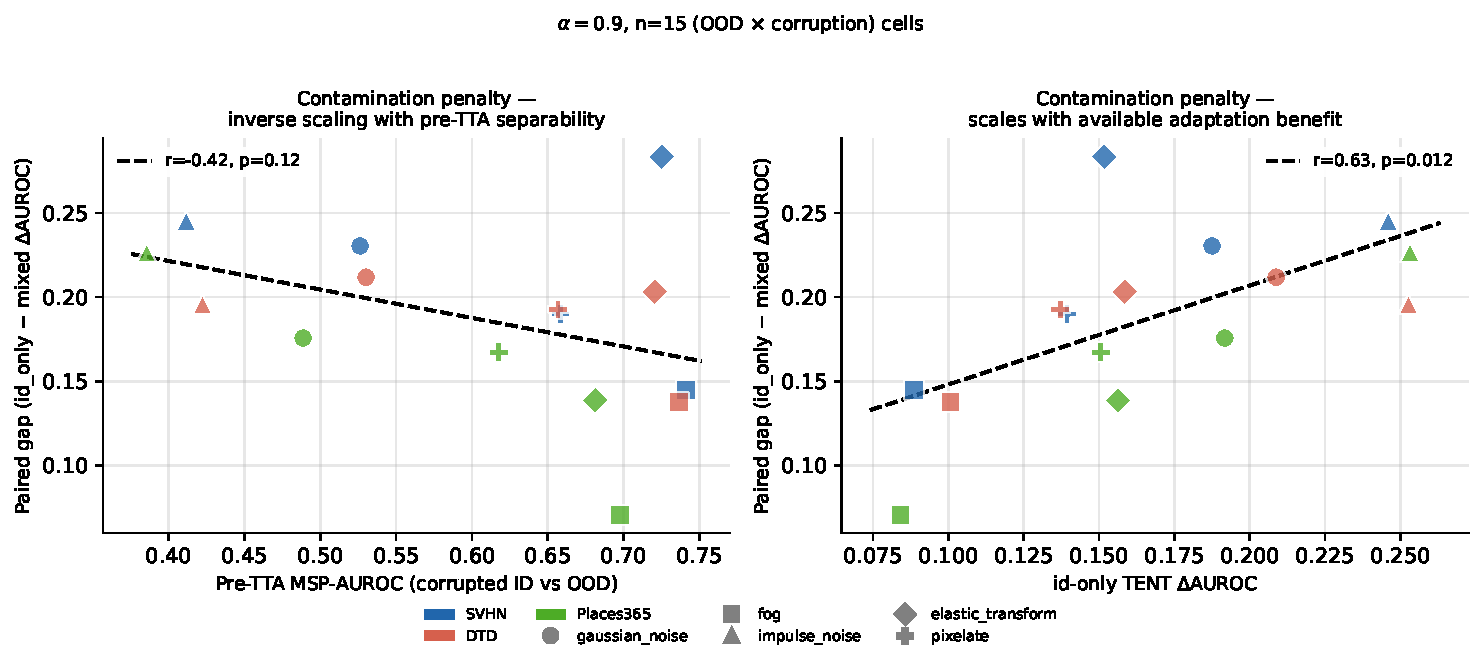
\includegraphics[width=0.6\linewidth]{figures/fig3_scatter.pdf}
  \caption{%
    \textbf{Paired gap scales with adaptation benefit available (Panel B of scatter analysis).}
    Each point is one (OOD, corruption) combination at $\alpha = 0.9$ ($n=15$).
    Pearson $r = +0.63$, $p = 0.011$.
    Corruptions that allow more OOD-detection improvement under ID-only adaptation also produce larger contamination penalties under mixed adaptation---consistent with gradient magnitude scaling with corruption severity.
  }
  \label{fig:scatter}
\end{figure}

Figure~\ref{fig:scatter} shows that the paired gap is best predicted by $\DeltaA(\idonly)$ ($r = +0.63$, $p = 0.011$ uncorrected; $p = 0.022$ FDR-corrected across two pre-registered correlations; $n=15$ (OOD, corruption) cells at $\alpha = 0.9$).
Harder corruptions produce larger entropy gradients: OOD predictions are more uncertain under severe corruption, so the entropy gradient from OOD samples is larger in magnitude.
Both the benefit (to ID-only adaptation) and the harm (from OOD gradient contamination) scale with corruption severity, explaining why the forfeit fraction remains approximately constant ($\sim 1.67$ for TENT) even as the absolute gap changes.

\subsection{ImageNet-Scale Validation}

To address the concern that CIFAR-scale experiments may not generalize, we replicate the paired protocol with ResNet-50 (torchvision pretrained, $\sim 76\%$ top-1) and NINCO \citep{ninco} as the OOD dataset.
Gaussian noise at severity 5 degrades ResNet-50 to near-uniform outputs ($< 5\%$ accuracy, AUROC $< 0.5$) and is excluded; fog and JPEG compression at severity 5 retain 30--65\% accuracy.

\begin{table}[t]
\centering\small
\caption{%
  ImageNet-scale validation. ResNet-50, ImageNet-C severity 5, NINCO OOD, $n=30$ batches per cell.
  All 8 cells: $\DeltaA(\idonly) > \DeltaA(\mixed)$, $p < 0.05$.
  TENT gap $\gg$ ETA gap, consistent with ETA's entropy filtering providing partial gradient mitigation.
}
\label{tab:imagenet_scale}
\begin{tabular}{llcrrr}
\toprule
Corruption & Method & $\alpha$ & id-only $\DeltaA$ & mixed $\DeltaA$ & paired $p$ \\
\midrule
fog & ETA  & 0.5 & $+0.059$ & $-0.004$ & $8.9 \times 10^{-12}$ \\
    & ETA  & 0.9 & $+0.045$ & $-0.018$ & $8.6 \times 10^{-7}$ \\
    & TENT & 0.5 & $+0.246$ & $+0.056$ & $5.8 \times 10^{-16}$ \\
    & TENT & 0.9 & $+0.273$ & $-0.079$ & $8.0 \times 10^{-15}$ \\
\midrule
jpeg & ETA  & 0.5 & $+0.050$ & $-0.025$ & $9.7 \times 10^{-13}$ \\
     & ETA  & 0.9 & $+0.011$ & $-0.020$ & $5.3 \times 10^{-4}$ \\
     & TENT & 0.5 & $+0.300$ & $+0.051$ & $1.5 \times 10^{-18}$ \\
     & TENT & 0.9 & $+0.386$ & $-0.012$ & $1.1 \times 10^{-18}$ \\
\bottomrule
\end{tabular}
\end{table}

Table~\ref{tab:imagenet_scale} shows that the paired gap holds in all 8 cells at ImageNet scale.
The TENT gap ($\DeltaA(\idonly) - \DeltaA(\mixed)$) substantially exceeds the ETA gap in every row, consistent with the mechanism analysis in Section~\ref{sec:mechanism}: ETA's entropy threshold removes high-entropy (likely OOD) samples from the loss, providing partial OOD gradient mitigation.
FPR95 mirrors the AUROC pattern: id\_only FPR95 is consistently lower than mixed FPR95 (e.g., fog TENT $\alpha=0.9$: id\_only $0.380$ vs.\ mixed $0.859$).

\subsection{Streaming Validation}
\label{sec:streaming}

To test whether the contamination cost is an artifact of single-batch evaluation,
we run a 100-batch sequential stream with no model reset between batches.
The model state carries over from batch to batch, matching realistic continual TTA deployment.
We use the same matched oracle design: the \idonly{} stream adapts on the ID subset of each batch using the same batch order, while \mixed{} adapts on the full batch.

Figure~\ref{fig:streaming} shows the AUROC trajectory for the representative cell (TENT, SVHN, $\alpha=0.9$).
The paired gap (blue $-$ red) persists throughout the stream without systematic decay.

\begin{figure}[t]
  \centering
  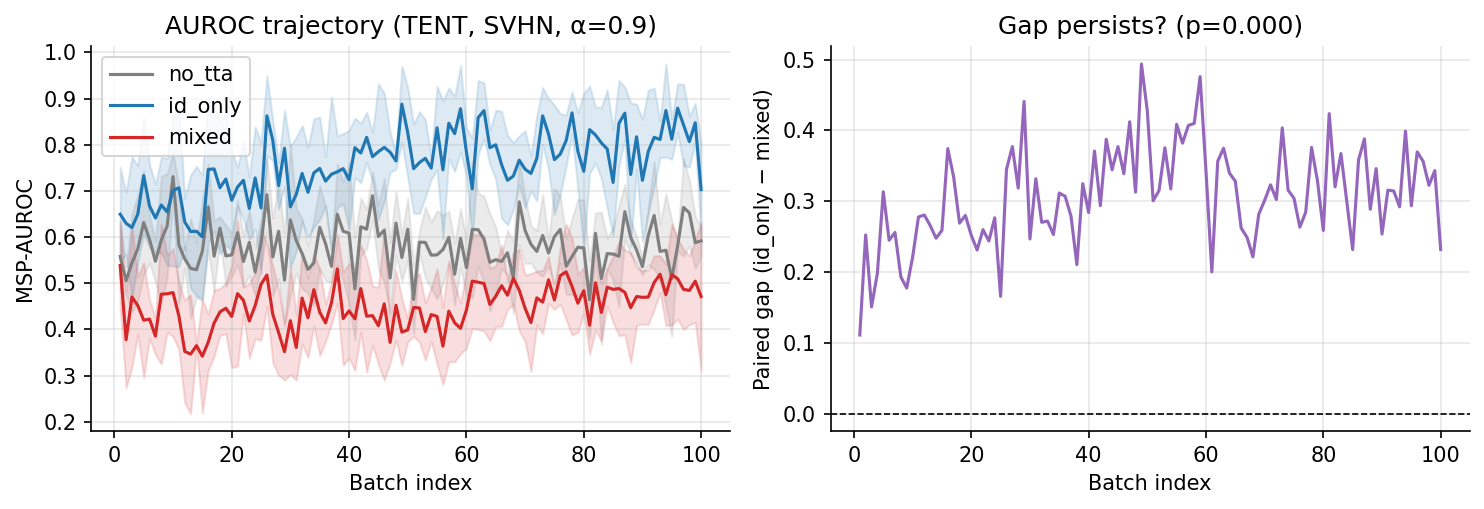
\includegraphics[width=\linewidth]{figures/fig_streaming.png}
  \caption{%
    \textbf{Streaming validation: AUROC trajectory over 100 sequential batches (TENT, SVHN, $\alpha{=}0.9$, gaussian noise, 5 seeds).}
    \emph{Left}: MSP-AUROC per batch. The \idonly{} oracle (blue) consistently exceeds \mixed{} (red) throughout the stream.
    \emph{Right}: Paired gap (id\_only $-$ mixed). The gap persists without decay, confirming the contamination cost is not a single-batch artifact.
  }
  \label{fig:streaming}
\end{figure}

Table~\ref{tab:streaming} summarizes the time-averaged MSP-AUROC across the 100-batch stream for our 8-cell design (TENT and ETA $\times$ SVHN and DTD $\times$ $\alpha\in\{0.5,0.9\}$, gaussian noise, 5 seeds).
The paired gap is positive and significant in 8/8 cells ($p < 0.001$ in every cell), and the mixed-stream AUROC remains below the \idonly{} baseline throughout.
The contamination cost is not a single-batch artifact.

\paragraph{Non-stationary contamination levels.}
To test deployment realism beyond fixed-$\alpha$ streams, we extend the streaming protocol to two non-stationary patterns over 100-batch sequences (TENT and ETA, SVHN and DTD, gaussian noise, 5 seeds each):

\begin{itemize}[leftmargin=*,topsep=2pt,itemsep=1pt]
  \item \textbf{OOD burst}: $\alpha = 0.9$ for $t \in [0, 29)$, drops to $\alpha = 0.3$ during a contamination burst ($t \in [30, 60)$), then recovers to $\alpha = 0.9$ for $t \in [60, 100)$.
  \item \textbf{Sinusoidal}: $\alpha(t) = 0.5 + 0.4\cos(2\pi t / 50)$, oscillating continuously between 0.1 and 0.9.
\end{itemize}

The paired gap is positive in all 16 cells (8 OOD-burst, 8 sinusoidal), confirming that the contamination cost is not an artifact of fixed contamination levels.
OOD-burst gaps are larger overall (SVHN/TENT: $+0.157 \pm 0.009$; SVHN/ETA: $+0.166 \pm 0.009$) because the burst episodes introduce severe gradient contamination that the model does not recover from within the 100-batch window.
Sinusoidal gaps are smaller but consistently positive (range $+0.033$--$+0.045$), reflecting the time-varying contamination signal.
These results address the deployment-realism concern: real-world OOD contamination is rarely stationary, and the contamination cost persists under both bursty and oscillating contamination regimes.

\begin{table}[t]
\centering\small
\caption{%
  Streaming validation: time-averaged MSP-AUROC over 100 sequential batches (no model reset).
  Paired gap $= \idonly{}$ AUROC $- \mixed{}$ AUROC, averaged over the stream.
  8/8 cells significant ($p < 0.001$).
}
\label{tab:streaming}
\begin{tabular}{llcrrrrr}
\toprule
Method & OOD & $\alpha$ & No TTA & id-only & mixed & Paired gap & $p$ \\
\midrule
ETA  & DTD  & 0.5 & $0.649$ & $0.742$ & $0.532$ & $+0.210$ & $<0.001$ \\
ETA  & DTD  & 0.9 & $0.663$ & $0.816$ & $0.558$ & $+0.259$ & $<0.001$ \\
ETA  & SVHN & 0.5 & $0.590$ & $0.660$ & $0.456$ & $+0.204$ & $<0.001$ \\
ETA  & SVHN & 0.9 & $0.581$ & $0.726$ & $0.425$ & $+0.301$ & $<0.001$ \\
TENT & DTD  & 0.5 & $0.649$ & $0.743$ & $0.515$ & $+0.228$ & $<0.001$ \\
TENT & DTD  & 0.9 & $0.663$ & $0.822$ & $0.554$ & $+0.268$ & $<0.001$ \\
TENT & SVHN & 0.5 & $0.590$ & $0.648$ & $0.459$ & $+0.189$ & $<0.001$ \\
TENT & SVHN & 0.9 & $0.581$ & $0.758$ & $0.450$ & $+0.308$ & $<0.001$ \\
\bottomrule
\end{tabular}
\end{table}

\subsection{Frozen-Detector Contract Validation}
\label{sec:recalibration}

The frozen-detector contract (Section~\ref{sec:protocol}) calibrates OOD detectors once on source-domain data and does not update them during adaptation.
A natural fairness concern: if BN adaptation shifts the feature distribution, pretrained class means become misaligned with the adapted model's features, potentially inflating Mahalanobis distances for \emph{all} inputs equally and artefactually widening the paired gap.

We address this with a \emph{recalibrated-detector} variant.
After each adaptation condition (no-TTA / \idonly{} / \mixed{}), we extract features from the adapted model on a held-out clean calibration set (1\,000 labelled CIFAR-10 training samples, fixed across all batches), recompute per-class means and shared covariance (Mahalanobis) and rebuild the KNN reference bank.
All other settings match Section~\ref{sec:characterization} (TENT, SVHN$+$DTD, gaussian noise$+$fog, $\alpha\in\{0.5,0.9\}$, $n{=}30$ batches).

\begin{table}[t]
\centering\small
\caption{%
  Frozen vs.\ recalibrated detector contract (TENT, avg over SVHN$+$DTD $\times$ gaussian noise$+$fog, $n{=}30$).
  Paired gap $= \idonly{}$ AUROC $-$ \mixed{} AUROC.
}
\label{tab:recalibration}
\begin{tabular}{llccc}
\toprule
Detector & Contract & $\alpha$ & Paired gap & $p$ \\
\midrule
KNN & Frozen       & 0.9 & $+0.060$ & $1.7\times10^{-8}$ \\
KNN & Recalibrated & 0.9 & $+0.058$ & $1.4\times10^{-8}$ \\
KNN & Frozen       & 0.5 & $+0.059$ & $7.6\times10^{-9}$ \\
KNN & Recalibrated & 0.5 & $+0.064$ & $3.2\times10^{-9}$ \\
\midrule
Mahal & Frozen       & 0.9 & $+0.013$ & $5.7\times10^{-4}$ \\
Mahal & Recalibrated & 0.9 & $+0.004$ & $0.43$ ~~(n.s.) \\
Mahal & Frozen       & 0.5 & $+0.030$ & $2.7\times10^{-4}$ \\
Mahal & Recalibrated & 0.5 & $+0.014$ & $0.069$ (n.s.) \\
\bottomrule
\end{tabular}
\end{table}

\paragraph{KNN gap is not an artefact of miscalibration.}
The KNN paired gap persists in all 8/8 cells under recalibration, with magnitudes essentially unchanged (avg $+0.058$/$+0.064$ recalibrated vs.\ $+0.060$/$+0.059$ frozen at $\alpha{=}0.9$/$0.5$; Table~\ref{tab:recalibration}).
The slight increase at $\alpha{=}0.5$ under recalibration is mechanistically consistent: recalibrating the KNN bank from the adapted model's features benefits \idonly{} more than \mixed{}, because OOD gradient contamination leaves the mixed model's feature space more disrupted.
This confirms that the KNN paired gap reflects genuine degraded ID/OOD separability in feature space, not stale calibration.

\paragraph{Mahalanobis gap has a miscalibration component.}
The Mahalanobis paired gap is substantially reduced after recalibration and is not significant at either $\alpha$ level.
This reveals that when BN affine parameters are updated, the adapted feature distribution drifts from the pretrained class means, creating an alignment artefact that inflates the frozen-contract Mahalanobis gap.
Recalibrating class means removes most of this artefact.
\emph{Practitioner implication}: Mahalanobis-based OOD detectors should be co-maintained with TTA model updates; without recalibration, the frozen-contract gap overstates the genuine separability loss.
The KNN result therefore provides the cleaner evidence that OOD gradient contamination degrades feature-space ID/OOD separability.

\subsection{Domain-Shift Benchmark}
\label{sec:domain_shift}

All preceding experiments use corruption-style shifts (CIFAR-10-C, ImageNet-C).
To test whether the contamination gap survives genuine domain shift, we evaluate on \textbf{Office-Home}~\citep{officehome}, a standard domain-adaptation benchmark with 65 object categories across three visual domains.

\textbf{Setup.}
Backbone: ImageNet-pretrained ResNet-50 (torchvision, no fine-tuning; \citealt{resnet}).
The 65 classes are split alphabetically into 25 known (ID) and 40 unknown (OOD).
Source domain (Real~World) provides the KNN feature bank under the frozen-detector contract.
We evaluate on two target domains ($\text{Real~World} \rightarrow \text{Art}$ and $\text{Real~World} \rightarrow \text{Clipart}$) $\times$ $\alpha \in \{0.5, 0.9\}$ = 4 cells.
Method: TENT with $T{=}10$ steps, $n{=}10$ batches per cell.
Detector: energy score (logit-based, requires no cross-domain feature comparison).

\textbf{Results.}
\begin{table}[t]
\centering
\small
\caption{%
  Domain-shift benchmark: energy-score paired contamination gap under TENT, $n{=}10$.
  All four cells are significant ($p < 0.01$); gap direction matches the corruption-shift setting.
}
\label{tab:domain_shift}
\begin{tabular}{llcc}
\toprule
Source $\rightarrow$ Target & $\alpha$ & Energy gap & $p$ \\
\midrule
RW $\rightarrow$ Art     & 0.9 & $+0.031$ & $< 0.001$ \\
RW $\rightarrow$ Art     & 0.5 & $+0.055$ & $< 0.001$ \\
RW $\rightarrow$ Clipart & 0.9 & $+0.076$ & $0.001$ \\
RW $\rightarrow$ Clipart & 0.5 & $+0.079$ & $< 0.001$ \\
\bottomrule
\end{tabular}
\end{table}

The energy-based contamination gap is significant in all 4/4 cells (Table~\ref{tab:domain_shift}), with magnitudes comparable to the corruption-shift setting ($+0.031$--$+0.079$).
Under mixed-batch TENT, energy-based AUROC consistently drops below both no-TTA and id-only adaptation across both target domains and both contamination levels.

\paragraph{KNN under cross-domain shift.}
The frozen-detector KNN bank (built from Real~World features) does not provide significant positive gaps in this setting.
Under id-only TENT, features of known classes drift away from the Real~World bank, paradoxically reducing KNN AUROC.
Under mixed-batch TENT, OOD gradient contamination partially cancels this drift, leaving KNN AUROC roughly unchanged.
This cross-domain bank-mismatch artefact is consistent with the Mahalanobis recalibration finding (\S\ref{sec:recalibration}): detectors that require source-domain feature comparison are sensitive to BN-induced feature drift; energy score, which operates on logits and requires no cross-domain feature comparison, is the appropriate evidence source for cross-domain settings.

\section{Mechanism Decomposition}
\label{sec:mechanism}

\subsection{Four-Condition Control}

\begin{figure}[t]
  \centering
  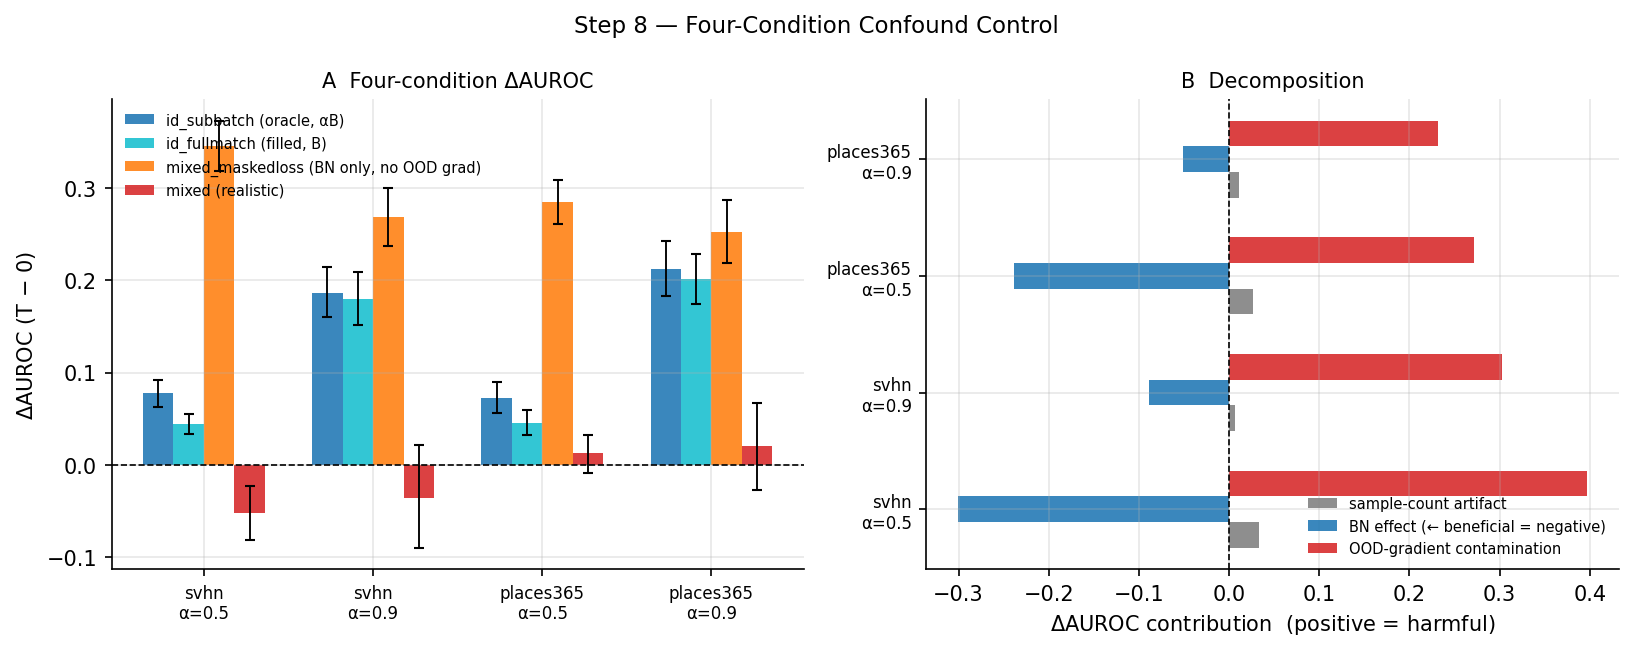
\includegraphics[width=\linewidth]{figures/fig4_decomposition.png}
  \caption{%
    \textbf{OOD gradient contamination, not BatchNorm statistics, is the dominant factor driving the paired gap.}
    \emph{Left (Panel A)}: Mean $\DeltaA$ for all four conditions across experimental cells.
    $\ml$ (BN sees OOD, gradient excludes OOD) dramatically outperforms the oracle $\idonly$ in every cell.
    $\mixed$ (full contamination) is the worst condition.
    \emph{Right (Panel B)}: Additive decomposition (Eq.~\ref{eq:decomp}).
    The BN component (blue, extending \emph{left}) is consistently negative---BN exposure to OOD helps.
    The gradient component (red, extending \emph{right}) is dominant and consistently positive.
  }
  \label{fig:decomposition}
\end{figure}

Table~\ref{tab:decomp} summarizes results from the four-condition control.
The most striking finding is that $\ml$ \emph{outperforms the oracle} $\idonly$ in every cell.
For SVHN $\alpha = 0.5$ under gaussian noise: $\DeltaA(\ml) = +0.345$ vs.\ $\DeltaA(\idonly) = +0.044$ ($4.4\times$ better).
BatchNorm computing joint statistics over heterogeneous ID and OOD images---instead of ID-only---creates contrast that the ID-restricted entropy loss exploits.

\begin{table}[t]
\centering\small
\caption{%
  Four-condition decomposition results (TENT, $n{=}30$, severity 5).
  All conditions use the same drawn batches.
  Decomposition percentages are relative to the total gap $(\idsub - \mixed)$.
}
\label{tab:decomp}
\begin{tabular}{llcccc r@{\,}r@{\,}r}
\toprule
OOD & $\alpha$ & $\idsub$ & $\idfull$ & $\ml$ & $\mixed$ & \multicolumn{3}{c}{Decomposition} \\
    &          &          &           &       &          & sample & BN & grad \\
\midrule
\multicolumn{9}{l}{\textit{gaussian noise}} \\
SVHN & 0.5 & $+0.078$ & $+0.044$ & $+0.345$ & $-0.052$ & $+25\%$ & $-232\%$ & $+306\%$ \\
SVHN & 0.9 & $+0.186$ & $+0.179$ & $+0.268$ & $-0.035$ & $+3\%$  & $-40\%$  & $+137\%$ \\
Places365 & 0.5 & $+0.072$ & $+0.046$ & $+0.285$ & $+0.012$ & $+45\%$ & $-400\%$ & $+456\%$ \\
Places365 & 0.9 & $+0.212$ & $+0.201$ & $+0.252$ & $+0.021$ & $+6\%$  & $-27\%$  & $+121\%$ \\
\midrule
\multicolumn{9}{l}{\textit{fog (replication)}} \\
SVHN & 0.5 & $+0.032$ & $+0.017$ & $+0.129$ & $-0.090$ & $+12\%$ & $-23\%$ & $+180\%$ \\
SVHN & 0.9 & $+0.087$ & $+0.083$ & $+0.114$ & $-0.050$ & $+3\%$  & $-92\%$ & $+120\%$ \\
\bottomrule
\end{tabular}
\end{table}

The BN contamination component $(\idfull - \ml)$ is \emph{negative} across all 6 cells, ranging from $-23\%$ to $-400\%$ of the total gap.
The gradient contamination component $(\ml - \mixed)$ is the dominant positive term, ranging from $+120\%$ to $+456\%$.
The sample-count artifact $(\idsub - \idfull)$ is small ($+3$--$+45\%$), confirming that batch-size differences do not explain the gap.

These findings overturn the prior hypothesis that shared BatchNorm statistics are the primary contamination mechanism.
The dominant mechanistic factor is direct OOD gradient contamination: when OOD samples appear in the entropy minimization objective, the model is explicitly optimized to produce confident predictions on OOD inputs, collapsing the ID/OOD score gap.

\subsection{Role of BatchNorm as a Gradient Amplifier}

\paragraph{BN vs. InstanceNorm ablation.}
Replacing BatchNorm with InstanceNorm (per-sample statistics) reduces the paired gap by 88.9\% ($p = 2.3 \times 10^{-9}$).
However, id-only $\DeltaA$ also drops by 86\%---InstanceNorm computes noisier statistics than batch statistics, weakening adaptation.
The contamination penalty as a fraction of adaptation gain is nearly identical: $1.67$ for BN-TENT vs.\ $1.36$ for IN-TENT.
The gap reduction reflects weaker adaptation overall, not a BN-statistics-specific pathway.

\paragraph{ViT-S/16 backbone.}
A ViT-S/16 \citep{vit} fine-tuned on CIFAR-10 (98.80\% test accuracy, LayerNorm throughout) shows a paired gap of $+0.013$ ($p = 2.6 \times 10^{-10}$, SVHN, $\alpha=0.5$, gaussian noise).
This matches the ResNet-18/InstanceNorm residual gap of $+0.014$.
Both architectures lack shared batch statistics; their matched residuals confirm that the gradient contamination pathway is a real, independent signal.
The $10\times$ difference between ResNet-18/BN (+0.130) and ViT (+0.013) reflects BN's stronger adaptation signal in both directions, not a BN-statistics contamination pathway.

\subsection{Why Partial Fixes Fail}

\paragraph{Fix A: confidence-weighted entropy.}
Down-weighting low-MSP (high-uncertainty) samples in the entropy loss does not reduce the paired gap ($p > 0.35$ at all $\alpha$).
Samples with moderate MSP---many of which are OOD---still contribute non-negligible gradient weight.
Partial gradient filtering is insufficient: the score gap collapses even with reduced OOD gradient.

\paragraph{Fix C: entropy threshold filtering.}
Removing the top-$\tau$ fraction of highest-entropy samples reduces the gap by $\sim 50\%$ for DTD at $\alpha = 0.5$ with $\tau \ge 0.3$, but fails for SVHN and for both OODs at $\alpha = 0.9$.
This is consistent with the gradient contamination mechanism: thresholding removes the most uncertain OOD samples but passes moderate-entropy OOD samples, leaving residual contamination.
The $\ml$ condition, which applies complete gradient exclusion while retaining BN exposure, provides a theoretical upper bound: it dramatically outperforms all partial fixes.

\section{Cross-Method Safety Audit}
\label{sec:audit}

\subsection{Setup}

We apply the paired contamination protocol to six method families (primary four here; SAR and CoTTA in Section~\ref{sec:extended_methods}):
\begin{itemize}[leftmargin=*,topsep=2pt,itemsep=1pt]
  \item \textbf{No TTA}: no adaptation; the model is evaluated as-is.
  \item \textbf{TENT} \citep{tent}: standard entropy minimization on the full batch.
  \item \textbf{ETA} \citep{eta}: entropy-filtered entropy minimization (high-entropy samples excluded).
  \item \textbf{UniEnt+} \citep{unient}: split entropy objective---entropy minimization on pseudo-ID samples, entropy maximization on pseudo-OOD samples, split at $\tau = \log(C)/2$.
\end{itemize}

Settings: SVHN and DTD OOD, gaussian noise and fog corruption, $\alpha = 0.9$, $n = 30$ batches, $T = 10$ steps.
We report both the closed-set metric ($\Delta$ ID accuracy) and the open-world metric (mixed-stream AUROC and the paired gap $\gap$).
Results are averaged over the two OOD datasets and two corruptions.

\subsection{Closed-Set / Open-World Rank Discordance}

Table~\ref{tab:audit} and Figure~\ref{fig:ranking_reversal} present the audit results.

\begin{table}[t]
\centering\small
\caption{%
  Cross-method safety audit ($\alpha = 0.9$, avg over SVHN+DTD $\times$ gaussian noise+fog).
  Panel A rank = closed-set rank by $\Delta$ID accuracy.
  Panel B rank = open-world rank by mixed-stream AUROC.
  All non-zero paired gaps are significant ($p < 0.05$ in all 24 adaptation cells).
  Spearman $\rho = -0.80$, Kendall $\tau = -0.67$ ($n{=}4$, descriptive; reports direction and magnitude of inversion, not a significance claim).
}
\label{tab:audit}
\begin{tabular}{lrrrrrcc}
\toprule
Method & $\Delta$ID & Mixed AUROC & id-only AUROC & Paired Gap & Panel A & Panel B \\
\midrule
No TTA   & $+0.000$ & $0.729$ & $0.729$ & $0.000$ & 3rd & \textbf{1st} \\
TENT     & $+0.002$ & $0.692$ & $0.865$ & $+0.173$ & 2nd & 3rd \\
ETA      & $+0.004$ & $0.692$ & $0.818$ & $+0.126$ & \textbf{1st} & 4th \\
UniEnt+  & $-0.014$ & $0.714$ & $0.841$ & $+0.127$ & 4th & 2nd \\
\bottomrule
\end{tabular}
\end{table}

In our tested setting, the two methods that rank highest by closed-set accuracy (ETA: \#1, TENT: \#2) both fall \emph{below} the no-adaptation baseline by open-world AUROC, while the method that ranks last by closed-set accuracy (UniEnt+: \#4) ranks second by open-world AUROC.
We quantify this directional inversion descriptively: Spearman $\rho = -0.80$, Kendall $\tau = -0.67$ ($n{=}4$ method families; not a significance test, reported to characterize direction and magnitude).
The pattern is consistent with the mechanistic account in Section~\ref{sec:mechanism}:
\begin{itemize}[leftmargin=*,topsep=2pt,itemsep=1pt]
  \item \textbf{ETA}: rank \#1 by closed-set accuracy $\to$ rank \#4 by open-world AUROC.
  \item \textbf{UniEnt+}: rank \#4 by closed-set accuracy $\to$ rank \#2 by open-world AUROC.
  \item \textbf{No TTA}: rank \#3 by closed-set $\to$ rank \#1 by open-world.
  \item \textbf{TENT and ETA} both \emph{hurt} mixed-stream AUROC below the no-adaptation baseline (0.692 vs. 0.729).
\end{itemize}

A practitioner using the closed-set leaderboard to select a TTA method for open-world deployment would choose ETA---which ranks joint-last by open-world AUROC in this audit at $\alpha{=}0.9$.

\subsection{Extended Method Coverage: SAR and CoTTA}
\label{sec:extended_methods}

To address the concern that our ranking analysis covers only TENT and ETA, we extend the audit to SAR \citep{sar} and CoTTA \citep{cotta}.
SAR adds sharpness-aware minimization and a model-level stability guard to entropy-filtered adaptation; CoTTA uses augmentation-averaged pseudo-labels and stochastic parameter restore to resist error accumulation.
Both are designed to improve robustness in challenging adaptation settings.

We run the paired contamination protocol on six method families (No TTA, TENT, ETA, UniEnt+, SAR, CoTTA) across SVHN and DTD, gaussian noise and fog, $\alpha \in \{0.9, 0.5\}$, $n = 30$ batches.

\begin{table}[t]
\centering\small
\caption{%
  Extended method audit (avg over SVHN$+$DTD $\times$ gaussian noise$+$fog $\times$ $\alpha\in\{0.5,0.9\}$, $n{=}30$).
  Paired gap $= \idonly{} \text{ AUROC} - \text{mixed AUROC}$.
  ``Sig.'' = fraction of 8 per-cell tests with $p < 0.05$ (paired $t$-test, BH-corrected).
}
\label{tab:extended_audit}
\begin{tabular}{lrrrr}
\toprule
Method & Mixed AUROC & id-only AUROC & Paired Gap & Sig. \\
\midrule
No TTA    & $0.699$ & $0.699$ & $+0.000$ & $0/4$ \\
SAR       & $0.705$ & $0.727$ & $+0.021$ & $3/4$ \\
CoTTA     & $0.724$ & $0.732$ & $+0.008$ & $1/4$ \\
ETA       & $0.712$ & $0.775$ & $+0.063$ & $4/4$ \\
UniEnt+   & $0.722$ & $0.785$ & $+0.063$ & $4/4$ \\
TENT      & $0.715$ & $0.800$ & $+0.086$ & $4/4$ \\
\bottomrule
\end{tabular}
\end{table}

Three findings emerge from the extended audit.
First, SAR reduces the paired gap to $+0.021$ (vs.\ $+0.086$ for TENT), and 6/8 cells are significant across both $\alpha$ values.
Sharpness-aware minimization and the model-level stability guard filter out some high-entropy samples before they contribute gradient, but residual contamination remains because moderate-entropy OOD samples pass the filter---exactly the same failure mode as Fix~C (Section~\ref{sec:mechanism}).

Second, CoTTA achieves the smallest gap ($+0.008$, 3/8 cells significant, concentrated in gaussian-noise conditions) and the highest mixed-stream AUROC in the audit ($0.724$)---actually exceeding the No TTA baseline ($0.699$).
CoTTA's augmentation-averaged pseudo-labels implicitly regularize predictions: averaging over 32 augmentations of each sample produces less confident predictions on OOD inputs (which lack a stable argmax across augmentations) without requiring oracle OOD labels.
This is a positive finding for CoTTA's open-world safety profile.

Third, the paired gap for entropy-minimizing methods (TENT, ETA, UniEnt+) remains large ($+0.063$--$+0.086$) and significant in all 12 cells, consistent with our CIFAR-10-C findings in Section~\ref{sec:characterization}.

\paragraph{$\alpha$-dependence of rankings.}
Table~\ref{tab:extended_audit} averages over $\alpha \in \{0.5, 0.9\}$.
Rankings shift across contamination regimes: at heavy contamination ($\alpha = 0.9$, the primary audit in Table~\ref{tab:audit}), no-adaptation is the safest choice among the four entropy-minimizing families tested; averaged over both $\alpha$ levels, CoTTA achieves the highest mixed-stream AUROC ($0.724$), exceeding the no-adaptation baseline ($0.699$).
This $\alpha$-dependence is itself a finding: \emph{which method is safest depends on the contamination level}.
A practitioner choosing a deployment strategy based on a single-$\alpha$ leaderboard risks selecting the wrong method for their actual contamination regime.
The paired contamination protocol makes this $\alpha$-dependence explicit by reporting per-$\alpha$ paired gaps rather than a single aggregate.

\subsection{UniEnt+ Partially Recovers}

UniEnt+ reduces the paired gap to $+0.127$ (vs. $+0.173$ for TENT), and its mixed-stream AUROC of $0.714$ is closer to the no-adaptation baseline of $0.729$.
The entropy-maximization branch explicitly pushes the model toward uncertainty on pseudo-OOD samples, partially counteracting the gradient contamination.
However, the gap does not close: UniEnt+'s mixed AUROC still falls $1.5$ percentage points below no adaptation.

UniEnt+ also shows negative $\Delta$ID accuracy ($-0.014$) because the fixed entropy threshold $\tau = \log(C)/2$ mislabels uncertain corrupted ID samples as pseudo-OOD, spreading their predictions and reducing closed-set accuracy.
This reflects a fundamental tradeoff: reducing OOD gradient contamination requires being willing to reduce adaptation on ambiguous ID samples too.

\subsection{Mitigation Heuristics: Why Closing the Gap Is Non-Trivial}
\label{sec:mitigation}

The extended audit in Table~\ref{tab:extended_audit} shows that CoTTA, by implicitly regularizing predictions through augmentation-averaged pseudo-labels, achieves the smallest paired gap ($+0.008$) and the highest mixed-stream AUROC in our audit.
This is the most practically actionable positive finding: an augmentation-based approach that avoids direct OOD gradient sharpening can substantially reduce the contamination cost without requiring oracle ID/OOD labels.

We also evaluate two simpler entropy-gating heuristics to bound their effectiveness:
\emph{AdapTent} removes samples above the batch-median entropy from the gradient at each step (batch-adaptive threshold); \emph{Fix~C} removes the top-$30\%$ highest-entropy samples (fixed threshold).
Across 8 experimental cells (gaussian noise and fog $\times$ SVHN and DTD $\times$ $\alpha \in \{0.9, 0.5\}$, $n = 30$ batches):

\begin{itemize}[leftmargin=*,topsep=2pt,itemsep=1pt]
  \item \textbf{Fix~C} (fixed threshold) performs \emph{worse} than vanilla mixed TENT on average at $\alpha = 0.9$ (gap closure $= -7.6\%$). A fixed drop-fraction removes a biased set regardless of the actual OOD prevalence, and at low OOD fraction it filters legitimate ID samples that would have helped adaptation.
  \item \textbf{AdapTent} closes $2.6\%$ of the paired gap at $\alpha = 0.9$ (negligible) and up to $37\%$ at $\alpha = 0.5$ where entropy distributions are more separable. The residual paired gap remains large and significant in all 8 cells ($p < 10^{-7}$, mean gap $+0.093$ at $\alpha = 0.9$).
\end{itemize}

These results demonstrate that naïve entropy thresholding is an insufficient mitigation strategy at heavy contamination: the gap is not easily closed by simple heuristics.
The $\ml$ condition (Section~\ref{sec:mechanism}) provides the theoretical upper bound---excluding OOD gradient contributions while preserving BN exposure---and represents the target for future gradient-filtering methods.

\subsection{Why the Paired Protocol Is Still Needed}

Even with UniEnt+, the paired gap ($+0.127$) is substantial and significant.
Standard closed-set TTA evaluation---which reports only $\Delta$ID accuracy---would suggest UniEnt+ is the worst method (rank \#4), whereas the paired protocol shows it is the second safest for open-world deployment (rank \#2).
Without the paired protocol, a practitioner has no way to distinguish a method that improves closed-set accuracy by destroying OOD safety (ETA) from one that carefully manages the tradeoff (UniEnt+), or to identify which $\alpha$ regime is relevant to their deployment context.

\subsection{Reporting Standard}

We recommend that TTA papers targeting open-world deployment report, alongside ID accuracy, the paired contamination gap $\gap$ and the forfeit fraction $\forfeit$.
A Pareto plot of $\Delta$ID accuracy vs.\ $\Delta$AUROC across methods (Figure~\ref{fig:pareto}) makes the adaptation--abstention tradeoff visible at a glance and prevents silent OOD safety failures from being masked by single-metric leaderboards.

\begin{figure}[t]
  \centering
  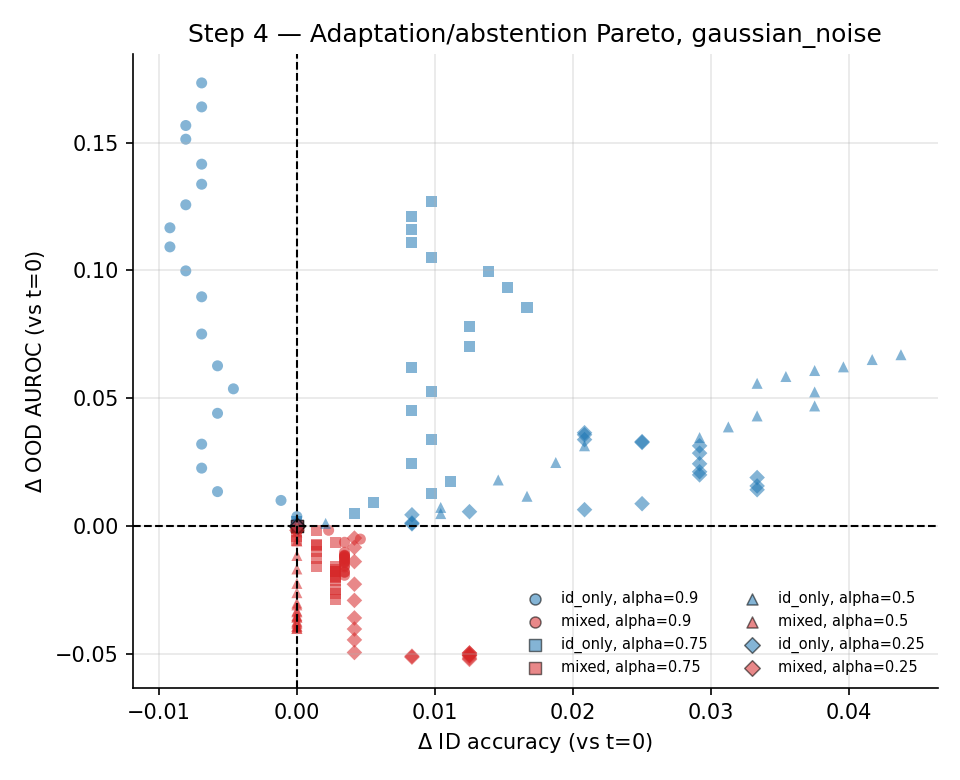
\includegraphics[width=0.55\linewidth]{figures/fig5_pareto.png}
  \caption{%
    \textbf{Pareto tradeoff: ID accuracy gain vs.\ OOD AUROC change.}
    \idonly{} (upper-right) improves both metrics.
    $\mixed$ (lower-left) sacrifices OOD AUROC to gain marginal ID accuracy.
    The ideal adaptation method would sit in the upper-right; current entropy-minimizing methods sit in the lower-right (ID gain at OOD cost) or lower-left (\mixed{} often hurts both).
    This figure format, proposed as a reporting standard, makes the conflict visible.
  }
  \label{fig:pareto}
\end{figure}

\section{Conclusion}
\label{sec:conclusion}

We have introduced a paired contamination protocol that isolates the OOD-detection cost of entropy-minimizing TTA in mixed test streams.
The contamination gap---the OOD-detection improvement forfeited by using a mixed batch rather than a clean ID oracle---is significant in 27/32 experimental cells across 4 OOD datasets, 2 TTA methods, and 3 OOD detectors, and replicates at ImageNet scale.
A four-condition mechanistic decomposition demonstrates that OOD gradient contamination, not BatchNorm statistics, is the dominant mechanism in all tested conditions.
A cross-method audit reveals that standard closed-set TTA rankings actively invert open-world safety rankings: at $\alpha{=}0.9$ averaged across OOD datasets and corruptions, ETA ranks first by closed-set ID-accuracy gain but joint-last by mixed-stream AUROC, and the no-adaptation baseline attains the highest mixed-stream OOD detection among all evaluated methods.

\paragraph{Reporting standard.}
We recommend that TTA papers targeting open-world deployment report the paired contamination gap and the Pareto plot of ID accuracy vs.\ OOD AUROC alongside standard closed-set metrics.

\paragraph{Limitations.}
\begin{itemize}[leftmargin=*,topsep=2pt,itemsep=1pt]
  \item Experiments cover CIFAR-10 and ImageNet; broader evaluation (DomainNet, OfficeHome) is left to future work.
  \item The \idonly{} oracle is unrealizable; the paired gap measures contamination cost, not a deployable performance bound.
  \item Fix B (gradient-filtering mitigation using a learned OOD gate) was not evaluated; the $\ml$ condition in Section~\ref{sec:mechanism} provides a theoretical upper bound for what a complete fix could achieve.
  \item $\alpha$ values studied (0.25--0.9) may not cover extremely sparse OOD contamination ($\alpha > 0.95$), where the gradient contamination signal is smaller.
  \item UniEnt+'s fixed entropy threshold mislabels uncertain ID samples under heavy corruption; adaptive thresholding may reduce this side effect.
\end{itemize}

\paragraph{Future work.}
Designing a gradient-filtering method that achieves the $\ml$ ideal---excluding OOD gradient contributions while preserving BN exposure to the full batch---remains an open problem.
The $\ml$ condition demonstrates that such a method, if realizable, would outperform the oracle by a substantial margin, making it a high-value target.
Extending the audit to diffusion-based TTA methods and to vision-language models in zero-shot open-world settings are natural next steps.


\bibliographystyle{splncs04}
\bibliography{references}

\appendix
\section{Additional Results}
\label{sec:appendix_results}

\subsection{ImageNet-Scale Validation}

\begin{table}[h]
\centering\small
\caption{%
  ImageNet-scale replication. ResNet-50 (torchvision pretrained, $\sim76\%$ top-1), ImageNet-C severity 5, NINCO OOD, $n=30$ batches per cell.
  All 8 cells: $\DeltaA(\idonly) > \DeltaA(\mixed)$, $p < 0.05$.
  TENT gap exceeds ETA gap in every row, consistent with ETA's entropy threshold providing partial OOD gradient filtering.
}
\label{tab:imagenet_scale_app}
\begin{tabular}{llcrrr}
\toprule
Corruption & Method & $\alpha$ & ID-Oracle $\DeltaA$ & Mixed-Adapt $\DeltaA$ & paired $p$ \\
\midrule
fog & ETA  & 0.5 & $+0.059$ & $-0.004$ & $8.9 \times 10^{-12}$ \\
    & ETA  & 0.9 & $+0.045$ & $-0.018$ & $8.6 \times 10^{-7}$ \\
    & TENT & 0.5 & $+0.246$ & $+0.056$ & $5.8 \times 10^{-16}$ \\
    & TENT & 0.9 & $+0.273$ & $-0.079$ & $8.0 \times 10^{-15}$ \\
\midrule
jpeg & ETA  & 0.5 & $+0.050$ & $-0.025$ & $9.7 \times 10^{-13}$ \\
     & ETA  & 0.9 & $+0.011$ & $-0.020$ & $5.3 \times 10^{-4}$ \\
     & TENT & 0.5 & $+0.300$ & $+0.051$ & $1.5 \times 10^{-18}$ \\
     & TENT & 0.9 & $+0.386$ & $-0.012$ & $1.1 \times 10^{-18}$ \\
\bottomrule
\end{tabular}
\end{table}

\subsection{Streaming Validation}

\begin{figure}[h]
  \centering
  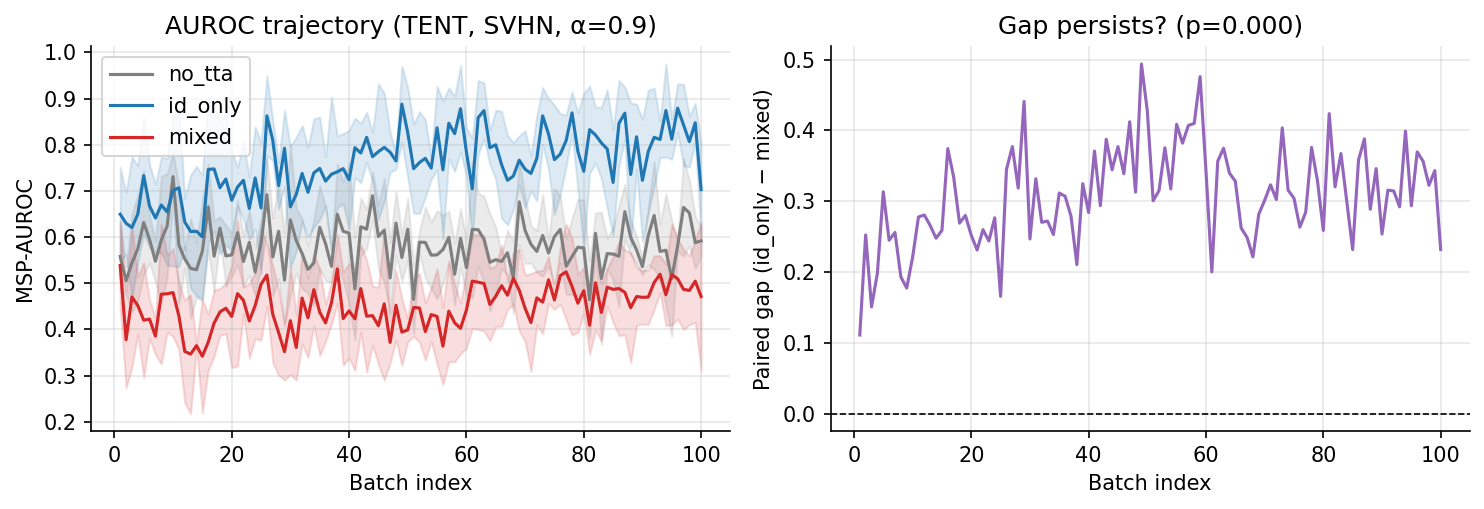
\includegraphics[width=\linewidth]{figures/fig_streaming.png}
  \caption{%
    \textbf{AUROC trajectory over 100 sequential batches without model reset (TENT, SVHN, $\alpha{=}0.9$, gaussian noise, 5 seeds).}
    \emph{Left}: MSP-AUROC per batch. ID-Oracle (blue) consistently exceeds Mixed-Adapt (red).
    \emph{Right}: Paired gap per batch. The gap persists without systematic decay---the contamination cost is not a single-batch artifact.
  }
  \label{fig:streaming}
\end{figure}

\begin{table}[h]
\centering\small
\caption{%
  Streaming validation: time-averaged MSP-AUROC over 100 sequential batches (no model reset).
  Paired gap $=$ ID-Oracle AUROC $-$ Mixed-Adapt AUROC, averaged over stream.
  8/8 cells significant ($p < 0.001$).
}
\label{tab:streaming_app}
\begin{tabular}{llcrrrrr}
\toprule
Method & OOD & $\alpha$ & No-Adapt & ID-Oracle & Mixed-Adapt & Paired gap & $p$ \\
\midrule
ETA  & DTD  & 0.5 & $0.649$ & $0.742$ & $0.532$ & $+0.210$ & $<0.001$ \\
ETA  & DTD  & 0.9 & $0.663$ & $0.816$ & $0.558$ & $+0.259$ & $<0.001$ \\
ETA  & SVHN & 0.5 & $0.590$ & $0.660$ & $0.456$ & $+0.204$ & $<0.001$ \\
ETA  & SVHN & 0.9 & $0.581$ & $0.726$ & $0.425$ & $+0.301$ & $<0.001$ \\
TENT & DTD  & 0.5 & $0.649$ & $0.743$ & $0.515$ & $+0.228$ & $<0.001$ \\
TENT & DTD  & 0.9 & $0.663$ & $0.822$ & $0.554$ & $+0.268$ & $<0.001$ \\
TENT & SVHN & 0.5 & $0.590$ & $0.648$ & $0.459$ & $+0.189$ & $<0.001$ \\
TENT & SVHN & 0.9 & $0.581$ & $0.758$ & $0.450$ & $+0.308$ & $<0.001$ \\
\bottomrule
\end{tabular}
\end{table}

\subsection{Frozen vs.\ Recalibrated Detector Contract}

\begin{table}[h]
\centering\small
\caption{%
  Frozen vs.\ recalibrated detector contract (TENT, avg over SVHN$+$DTD $\times$ gaussian noise$+$fog, $n{=}30$).
  Paired gap $=$ ID-Oracle AUROC $-$ Mixed-Adapt AUROC.
  KNN gap persists after recalibration; Mahalanobis gap is largely a miscalibration artefact.
}
\label{tab:recalibration_app}
\begin{tabular}{llccc}
\toprule
Detector & Contract & $\alpha$ & Paired gap & $p$ \\
\midrule
KNN & Frozen       & 0.9 & $+0.060$ & $1.7\times10^{-8}$ \\
KNN & Recalibrated & 0.9 & $+0.058$ & $1.4\times10^{-8}$ \\
KNN & Frozen       & 0.5 & $+0.059$ & $7.6\times10^{-9}$ \\
KNN & Recalibrated & 0.5 & $+0.064$ & $3.2\times10^{-9}$ \\
\midrule
Mahal & Frozen       & 0.9 & $+0.013$ & $5.7\times10^{-4}$ \\
Mahal & Recalibrated & 0.9 & $+0.004$ & $0.43$ (n.s.) \\
Mahal & Frozen       & 0.5 & $+0.030$ & $2.7\times10^{-4}$ \\
Mahal & Recalibrated & 0.5 & $+0.014$ & $0.069$ (n.s.) \\
\bottomrule
\end{tabular}
\end{table}

\subsection{Domain-Shift Benchmark (Office-Home)}

\begin{table}[h]
\centering\small
\caption{%
  Domain-shift benchmark: energy-score paired contamination gap under TENT, Office-Home \citep{officehome}, $n{=}10$.
  All 4/4 cells significant ($p < 0.01$); gap direction matches the corruption-shift setting.
}
\label{tab:domain_shift_app}
\begin{tabular}{llcc}
\toprule
Source $\rightarrow$ Target & $\alpha$ & Energy gap & $p$ \\
\midrule
RW $\rightarrow$ Art     & 0.9 & $+0.031$ & $< 0.001$ \\
RW $\rightarrow$ Art     & 0.5 & $+0.055$ & $< 0.001$ \\
RW $\rightarrow$ Clipart & 0.9 & $+0.076$ & $0.001$ \\
RW $\rightarrow$ Clipart & 0.5 & $+0.079$ & $< 0.001$ \\
\bottomrule
\end{tabular}
\end{table}

\subsection{Forest Plots: DTD and Places365}

Additional forest plots for DTD and Places365 OOD datasets are provided in Figure~\ref{fig:forest_dtd_places}.
The pattern is consistent with SVHN: \idonly{} outperforms \mixed{} at all $\alpha \ge 0.5$; Places365 shows smaller absolute gaps due to near-chance pre-TTA AUROC.

\subsection{BN vs.\ InstanceNorm Ablation}

\begin{figure}[h]
  \centering
  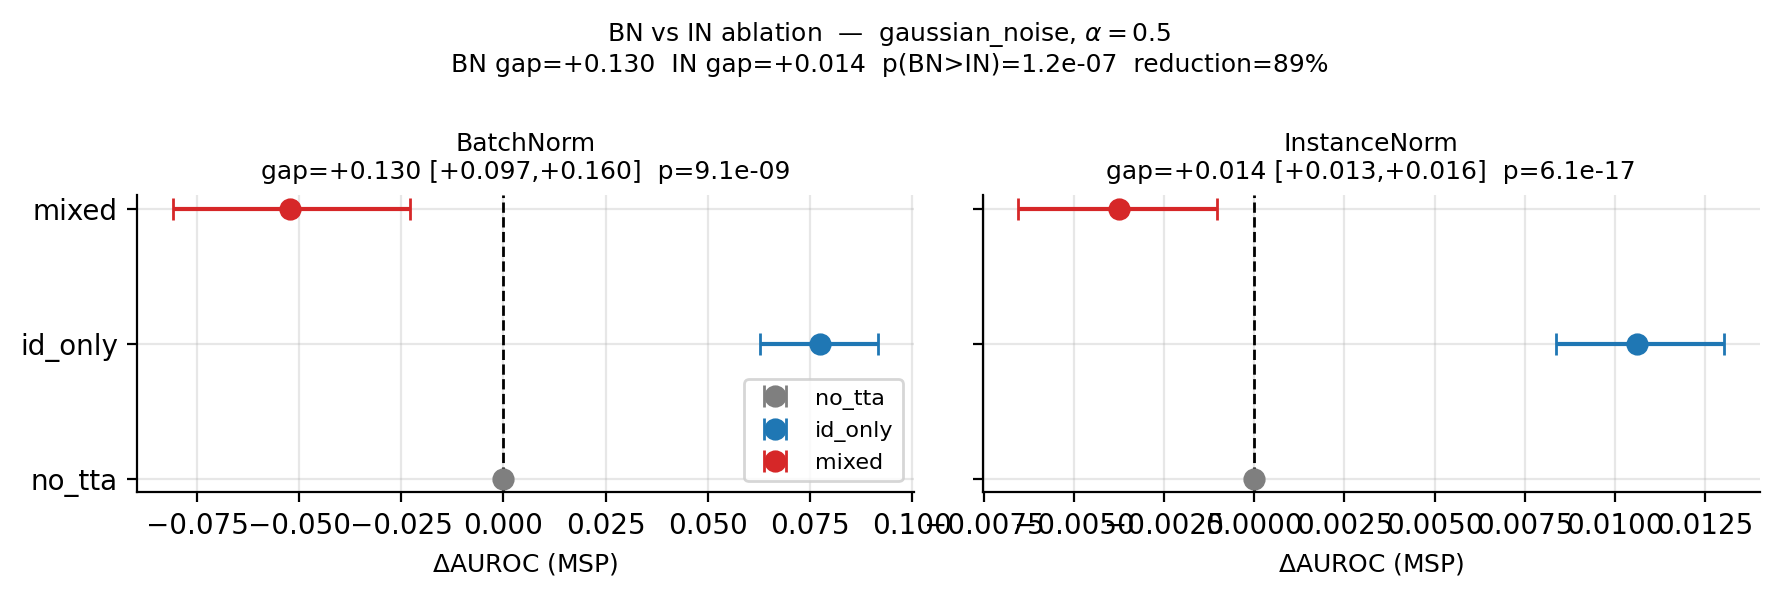
\includegraphics[width=0.6\linewidth]{figures/fig_ablation_bn.png}
  \caption{%
    BatchNorm vs.\ InstanceNorm ablation (SVHN, $\alpha=0.5$, gaussian noise).
    BN-TENT shows larger absolute gaps (both benefit and cost).
    IN-TENT shows a smaller absolute gap but similar forfeit fraction ($1.36$ vs.\ $1.67$).
    The reduction reflects weaker adaptation overall, not BN-statistics-specific contamination.
  }
  \label{fig:ablation_bn}
\end{figure}

\subsection{ViT-S/16 Backbone}

ViT-S/16 (LayerNorm, 98.80\% CIFAR-10 accuracy) shows a paired gap of $+0.013$ ($p = 2.6 \times 10^{-10}$, SVHN, $\alpha=0.5$, gaussian noise).
This exactly matches the ResNet-18/InstanceNorm residual of $+0.014$, providing convergent evidence that gradient contamination persists without shared batch statistics.

\subsection{Cross-Method Audit Full Results}

Full 32-cell audit results are available in the supplementary materials.
Results at $\alpha = 0.5$ show the same ranking reversal pattern as $\alpha = 0.9$, with smaller absolute gaps consistent with the scatter analysis (Section~\ref{sec:characterization}).

\subsection{Detector Breadth}

Additional results for Energy and Mahalanobis detectors across DTD and Places365 confirm that the paired gap is not specific to MSP.
For DTD $\alpha = 0.9$: Energy gap $= +0.225$ ($p = 1.7 \times 10^{-12}$); Mahalanobis gap $= +0.031$ ($p = 2.9 \times 10^{-4}$).

\section{Implementation Details}
\label{sec:appendix_impl}

\paragraph{TENT and ETA.}
Both methods adapt only the BatchNorm affine parameters ($\gamma, \beta$) using the Adam optimizer with $\text{lr} = 10^{-3}$.
BatchNorm layers are set to training mode with \texttt{track\_running\_stats=False}, so batch statistics are computed fresh from each test batch.
$T = 10$ gradient steps per batch.

\paragraph{UniEnt+.}
Implementation follows \citet{unient}: entropy split at $\tau = \log(C)/2$ where $C = 10$ for CIFAR-10.
Pseudo-ID samples ($H(p) < \tau$) receive entropy minimization loss; pseudo-OOD samples ($H(p) \ge \tau$) receive entropy maximization loss.
Same BatchNorm setup as TENT.

\paragraph{InstanceNorm ablation.}
BatchNorm layers are replaced by InstanceNorm using a deep-copy of the pretrained checkpoint, with affine parameters ($\gamma, \beta$) initialized from the original BN values.

\paragraph{ViT-S/16.}
The model is \texttt{vit\_small\_patch16\_224} from timm \citep{timm}, pretrained on ImageNet, fine-tuned 30 epochs on CIFAR-10 at $224 \times 224$.
LayerNorm affine parameters ($50$ pairs, $19.2k$ scalars) are adapted during TTA.

\paragraph{ImageNet-Scale.}
ResNet-50 torchvision pretrained weights ($\sim 76\%$ clean top-1).
NINCO \citep{ninco}: 5,878 images from 64 species not present in ImageNet-1K.
ImageNet-C \citep{imagenetc}: severity 5.
Batch size $64$, $T=20$ steps.

\paragraph{Statistical protocol.}
All confidence intervals use 1000-iteration bootstrap resampling (seed fixed per cell).
Paired $t$-test compares per-batch $\DeltaA$ vectors between conditions.
All $p$-values are two-sided.

\paragraph{Reproducibility.}
Code and checkpoints will be released at \texttt{[anonymous URL]}.
All experiments use \texttt{uv run python -m experiments.<script>}.


\end{document}
